% Copyright (c) 2025 Rafig Huseynzade. All Rights Reserved.
% Licensed under CC BY-NC-ND 4.0
% Original work - do not copy without attribution

\documentclass[11pt]{article}
\usepackage{amsmath, amssymb}
\usepackage{amsthm}
\usepackage{tikz}
\usepackage{hyperref}
\usepackage{geometry}
\usepackage{mathtools}
\usepackage{graphicx}
\usepackage{float}
\usepackage{subcaption}

\geometry{margin=1in}

% Theorem environments
\newtheorem{theorem}{Theorem}[section]
\newtheorem{lemma}[theorem]{Lemma}
\newtheorem{proposition}[theorem]{Proposition}
\newtheorem{corollary}[theorem]{Corollary}
\theoremstyle{definition}
\newtheorem{definition}[theorem]{Definition}
\newtheorem{example}[theorem]{Example}
\newtheorem{remark}[theorem]{Remark}

% Convenience macros
\newcommand{\PSi}{\Psi}
\newcommand{\iotaK}{\iota_k}
\newcommand{\PsiPk}{\PSi\text{-}P_k}
\newcommand{\PsiNPk}{\PSi\text{-}NP_k}
\newcommand{\PsiPSPACEk}{\PSi\text{-}PSPACE_k}
\newcommand{\bits}{\{0,1\}}
\newcommand{\len}[1]{\left|#1\right|}
\newcommand{\ceil}[1]{\left\lceil #1 \right\rceil}
\renewcommand{\checkmark}{$\surd$}

\title{Psi-TM: Minimal Introspection for Complexity Barrier Bypass\\
\large{A Complete Mathematical Foundation for Introspective Computation}}

\author{Rafig Huseynzade\\
Arizona State University\\
\href{mailto:huseynzaderafig@gmail.com}{huseynzaderafig@gmail.com}}

\date{\today}

\begin{document}

\maketitle

\begin{abstract}
We introduce Psi-TM ($\Psi$-TM), a computational model that extends Structurally-Aware Turing Machines (SA-TM) with minimal constant-depth introspection $k = O(1)$. We prove that Psi-TM bypasses all four classical complexity barriers while maintaining equivalence to standard Turing machines in computational power. Our main result establishes $P^{O_\Psi}_\Psi \neq NP^{O_\Psi}_\Psi$ for a specifically constructed oracle $O_\Psi$, demonstrating that minimal self-reflection suffices for complexity separation. 

We further establish a strict hierarchy of minimal introspection requirements: relativization requires $k \geq 1$, natural proofs and proof complexity require $k \geq 2$, and algebraization requires $k \geq 3$. The optimal design with $k = 3$ provides complete barrier bypass with minimal introspection. This work bridges the gap between theoretical barrier bypass and practical computational models, opening new directions in complexity theory.
\end{abstract}

\tableofcontents
\newpage

\section{Introduction}

The pursuit of resolving $P$ vs $NP$ has encountered four fundamental barriers: relativization \cite{BGS75}, natural proofs \cite{RR97}, algebraization \cite{AW09}, and proof complexity. Structurally-Aware Turing Machines (SA-TM) \cite{SA-TM} demonstrated that self-reflective computation can bypass these barriers, but at the cost of potentially unlimited introspection capabilities.

We introduce Psi-TM ($\Psi$-TM), which constrains SA-TM introspection to constant depth $k = O(1)$ while preserving barrier bypass capabilities. This creates a "natural" computational model that appears equivalent to standard Turing machines but possesses sufficient structural awareness for complexity separation.

\textbf{Our Contributions:}
\begin{enumerate}
\item \textbf{Formal Model:} Complete 7-tuple specification of Psi-TM with $k$-limited introspection
\item \textbf{Main Result:} Oracle separation $P^{O_\Psi}_\Psi \neq NP^{O_\Psi}_\Psi$ via diagonalization
\item \textbf{Barrier Analysis:} Systematic bypass of all four classical complexity barriers
\item \textbf{Computational Equivalence:} Polynomial simulation between Psi-TM and standard TMs
\item \textbf{Minimality Analysis:} Strict hierarchy of minimal $k$ requirements for barrier bypass
\item \textbf{Optimal Design:} $k=3$ provides complete barrier bypass with minimal introspection
\end{enumerate}

\section{The Psi-TM Model}

\subsection{Formal Definition of Structural Depth}

\begin{definition}[Binary Tree]
A binary tree $T$ is a finite tree where each node has at most two children. We denote:
\begin{itemize}
\item $\text{root}(T)$ -- the root node of $T$
\item $\text{left}(v)$ -- the left child of node $v$ (if exists)
\item $\text{right}(v)$ -- the right child of node $v$ (if exists)
\item $\text{leaf}(T)$ -- the set of leaf nodes in $T$
\item $\text{depth}(v)$ -- the depth of node $v$ (distance from root)
\item $\text{depth}(T) = \max_{v \in T} \text{depth}(v)$ -- the depth of tree $T$
\end{itemize}
\end{definition}

\begin{definition}[Parsing Tree]
For a string $w \in \{0,1\}^*$, a parsing tree $T_w$ is a binary tree where:
\begin{itemize}
\item Each leaf is labeled with a symbol from $\{0,1\}$
\item Each internal node represents a structural composition
\item The concatenation of leaf labels in left-to-right order equals $w$
\end{itemize}
\end{definition}

\begin{definition}[Formal Structural Depth]
For a string $w \in \{0,1\}^*$, the structural depth $d(w)$ is defined as:
$$d(w) = \min_{T_w} \text{depth}(T_w)$$
where the minimum is taken over all possible parsing trees $T_w$ for $w$.

\textbf{Base cases:}
\begin{itemize}
\item $d(\varepsilon) = 0$ (empty string)
\item $d(0) = d(1) = 0$ (single symbols)
\end{itemize}

\textbf{Recursive case:}
For $|w| > 1$, $d(w) = \min_{w=uv} \{1 + \max(d(u), d(v))\}$ where the minimum is taken over all binary partitions of $w$.
\end{definition}

\begin{lemma}[Well-Definedness of Structural Depth]
The structural depth function $d: \{0,1\}^* \to \mathbb{N}$ is well-defined and computable in $O(n^3)$ time using dynamic programming.
\end{lemma}

\begin{proof}
\textbf{Well-Definedness:}
\begin{enumerate}
\item For strings of length $\leq 1$, $d(w)$ is explicitly defined
\item For longer strings, the minimum exists because:
  \begin{itemize}
  \item The set of possible partitions is finite (at most $n-1$ partitions for length $n$)
  \item Each partition yields a finite depth value
  \item The minimum of a finite set of natural numbers exists
  \end{itemize}
\end{enumerate}

\textbf{Computability:}
We provide a dynamic programming algorithm:

\textbf{Algorithm: Structural Depth Computation}

\textbf{Input:} String $w = w_1w_2\ldots w_n$

\textbf{Output:} Structural depth $d(w)$

\begin{enumerate}
\item Initialize $dp[i][j] = 0$ for all $i \leq j$
\item For $i = 1$ to $n$:
   \begin{itemize}
   \item $dp[i][i] = 0$ (Base case: single symbols)
   \end{itemize}
\item For $\text{len} = 2$ to $n$:
   \begin{itemize}
   \item For $i = 1$ to $n-\text{len}+1$:
      \begin{itemize}
      \item $j = i + \text{len} - 1$
      \item $dp[i][j] = \infty$
      \item For $k = i$ to $j-1$:
         \begin{itemize}
         \item $dp[i][j] = \min(dp[i][j], 1 + \max(dp[i][k], dp[k+1][j]))$
         \end{itemize}
      \end{itemize}
   \end{itemize}
\item Return $dp[1][n]$
\end{enumerate}

\textbf{Correctness:}
\begin{enumerate}
\item Base cases are handled correctly
\item For each substring $w[i:j]$, we try all possible binary partitions
\item The algorithm computes the minimum depth over all parsing trees
\item Time complexity: $O(n^3)$ due to three nested loops
\end{enumerate}
\end{proof}

\subsection{Formal Definition}

\begin{definition}[Psi-TM]
A Psi-TM is a 7-tuple:
$$M_\Psi = (Q, \Sigma, \Gamma, \delta, q_0, F, \iota_k)$$
where:
\begin{itemize}
\item $(Q, \Sigma, \Gamma, \delta, q_0, F)$ is a deterministic Turing machine
\item $\iota_k: \Gamma^* \times \Gamma^* \times \mathbb{N} \to \Psi_k$ is $k$-limited introspection
\item $\Psi_k$ denotes structural metadata of depth $\leq k$
\item $k = O(1)$ is a constant
\end{itemize}
\end{definition}

\begin{definition}[Transition Function]
The extended transition function is:
$$\delta: Q \times \Gamma \times \Psi_k \to Q \times \Gamma \times \{L, R, S\}$$
where $\Psi_k$ provides structural metadata accessible through introspection calls.
\end{definition}

\begin{definition}[Configuration]
A Psi-TM configuration is a tuple:
$$\mathcal{C} = (q, \alpha, \beta, \psi)$$
where $q \in Q$, $\alpha, \beta \in \Gamma^*$ represent tape content, and $\psi \in \Psi_k$ is the introspective state.
\end{definition}

\subsection{Formal Introspection Functions}

\begin{definition}[Formal INT\_PATTERN(k)]
The function $\texttt{INT\_PATTERN(k)}: \Gamma^* \times \mathbb{N} \to 2^{\text{Patterns}_k}$ is defined as:
$$\texttt{INT\_PATTERN(k)}(w) = \{(i,j,T) \mid w[i:j] \text{ has parsing tree } T \text{ with depth } \leq k\}$$
where $\text{Patterns}_k$ is the set of all structural patterns of depth $\leq k$.
\end{definition}

\begin{definition}[Formal INT\_STRUCT(k)]
The function $\texttt{INT\_STRUCT(k)}: \Gamma^* \times \mathbb{N} \to \text{Struct}_k$ is defined as:
$$\texttt{INT\_STRUCT(k)}(w) = \{\text{depth}(T) \mid T \text{ is a parsing tree for } w \text{ with depth } \leq k\}$$
where $\text{Struct}_k$ is the set of structural depth information up to level $k$.
\end{definition}

\begin{definition}[Introspective Function]
The function $\iota_k: \Gamma^* \times \Gamma^* \times \mathbb{N} \to \Psi_k$ defines introspective metadata:
$$\iota_k(\alpha, \beta, k) = (\texttt{INT\_PATTERN(k)}(\alpha), \texttt{INT\_PATTERN(k)}(\beta), \texttt{INT\_STRUCT(k)}(\alpha \cdot \beta))$$
where $k$ is the limitation on introspection depth, and $\psi$ contains only structural information of depth at most $k$.
\end{definition}

\begin{definition}[k-Limited Introspection]
Introspection is called k-limited if for any $\alpha, \beta \in \Gamma^*$:
$$|\iota_k(\alpha, \beta, k)| \leq f(k) \cdot (|\alpha| + |\beta|)$$
where $f: \mathbb{N} \to \mathbb{N}$ is a polynomial function, and $\iota_k$ cannot access the complete tape content, only structural patterns of depth $k$.
\end{definition}

\begin{lemma}[Information Limitation]
For any $k \geq 1$, there exist strings $w_1, w_2 \in \{0,1\}^*$ such that:
\begin{enumerate}
\item $d(w_1) = k+1$ and $d(w_2) = k$
\item $\iota_k(w_1, \varepsilon, k) = \iota_k(w_2, \varepsilon, k)$
\end{enumerate}
\end{lemma}

\begin{proof}
We construct specific strings $w_1$ and $w_2$ that demonstrate this limitation.

\textbf{Construction:}
\begin{enumerate}
\item Let $w_1$ be a string with structural depth $k+1$ (e.g., a balanced binary tree of depth $k+1$)
\item Let $w_2$ be a string with structural depth $k$ (e.g., a balanced binary tree of depth $k$)
\item Both strings have identical structure up to level $k$
\item The difference appears only at level $k+1$ in $w_1$
\end{enumerate}

\textbf{Proof of Equality:}
Since $\texttt{INT\_PATTERN(k)}$ and $\texttt{INT\_STRUCT(k)}$ only access information up to depth $k$:
\begin{align*}
\iota_k(w_1, \varepsilon, k) &= (\texttt{INT\_PATTERN(k)}(w_1), \texttt{INT\_PATTERN(k)}(\varepsilon), \texttt{INT\_STRUCT(k)}(w_1)) \\
&= (\texttt{INT\_PATTERN(k)}(w_2), \texttt{INT\_PATTERN(k)}(\varepsilon), \texttt{INT\_STRUCT(k)}(w_2)) \\
&= \iota_k(w_2, \varepsilon, k)
\end{align*}

This demonstrates that introspection depth $k$ cannot distinguish between strings of different structural depths beyond level $k$.
\end{proof}

\subsection{Introspection API}

\begin{table}[ht]
\centering
\caption{Psi-TM Introspection API}
\label{tab:introspection-api}
\begin{tabular}{|l|l|l|l|}
\hline
\textbf{Function} & \textbf{Parameters} & \textbf{Returns} & \textbf{Constraint} \\
\hline
$\texttt{INT\_STATE()}$ & None & Current state $q \in Q$ & $k \geq 1$ \\
\hline
$\texttt{INT\_CODE(i)}$ & Index $i \in \mathbb{Z}$ & Code symbol $\delta[i]$ & $|i| \leq k$ \\
\hline
$\texttt{INT\_INPUT(j)}$ & Position $j \in \mathbb{N}$ & Input symbol at position $j$ & $|j| \leq k$ \\
\hline
$\texttt{INT\_STRUCT(d)}$ & Depth $d \in \mathbb{N}$ & Structural patterns at depth $d$ & $d \leq k$ \\
\hline
\multicolumn{4}{|c|}{\textbf{Key Constraint: $k = O(1)$ ensures bounded introspection}} \\
\hline
\end{tabular}
\end{table}

The key constraint $k = O(1)$ ensures that introspection accesses only a constant amount of structural information, independent of input size.

\section{Formal Semantics and Budgets (v0.6)}

This section fixes the formal semantics of introspection and its resource accounting. All later results that reason about the quantity of introspective information will cite Lemma~\ref{lem:one-step-budget} from this section.

\subsection{Coding of Structural Metadata}

\begin{definition}[Canonical integer code $\gamma$]
\label{def:gamma}
For $m\in\mathbb{N}_{\ge1}$, let $\gamma(m)$ be the Elias gamma code: $\gamma(m)=0^{b}\,1\,\mathrm{bin}(m\bmod 2^{b})$, where $b=\lfloor\log_2 m\rfloor$ and $\mathrm{bin}(\cdot)$ is the $b$-bit binary expansion. Then $\gamma$ is prefix-free and $|\gamma(m)|=2\lfloor\log_2 m\rfloor+1\le 2\log_2 m + 1$.
\end{definition}

\begin{proof}
No codeword is a prefix of another because the unary prefix $0^{b}1$ uniquely determines the boundary before the $b$ data bits. Length follows by definition. \qed
\end{proof}

\begin{definition}[Admissible metadata atoms]
\label{def:atoms}
Fix the finite tag set $\mathsf{Tag}=\{\textsf{state},\textsf{head},\textsf{win1},\ldots,\textsf{win}k\}$. An admissible atom is a pair $(\tau, v)$ where $\tau\in\mathsf{Tag}$ and $v\in\mathbb{N}$. For inputs of length $n$, we require $v\le n+2$ for $\tau\in\{\textsf{head},\textsf{win}d\}$ and $v\le |Q|$ for $\tau=\textsf{state}$.
\end{definition}

\begin{definition}[Canonical prefix-free code $C_k$ for $\PSi_k$]
\label{def:psi-k}
Let an item sequence be $(a_0,a_1,\ldots,a_r)$ with $r\in\{0,1,\ldots,k\}$ and each $a_i=(\tau_i,v_i)$ an admissible atom. Define
\[
C_k((a_i)_{i=0}^r)\;:=\; \gamma(r+1)\,\big\|\,\prod_{i=0}^{r}\Big(\mathrm{tag}(\tau_i)\,\big\|\,\gamma(v_i+1)\Big),
\]
where $\mathrm{tag}(\cdot)$ is a fixed 3-bit code for $\mathsf{Tag}$ and $\|$ denotes concatenation. The family $\PSi_k$ is the range of $C_k$ over all valid sequences for inputs of length $n$.
\end{definition}

\begin{lemma}[Prefix-freeness]
\label{lem:prefixfree}
The code $C_k$ is prefix-free.
\end{lemma}

\begin{proof}
The header $\gamma(r+1)$ is prefix-free and determines the exact number $r+1$ of items. Each item consists of a fixed-length tag followed by a self-delimiting $\gamma(v_i+1)$. Therefore boundaries are uniquely decodable and no codeword is a prefix of another. \qed
\end{proof}

\begin{lemma}[Length bound]
\label{lem:length-bound}
There exist absolute constants $\beta_0,\beta_1\in\mathbb{N}$ such that for all input lengths $n\ge1$ and $k\ge0$,
\[
\big|C_k((a_i)_{i=0}^{r})\big|\;\le\; \beta_0 + \beta_1\,k\,\lceil\log_2(n+2)\rceil.
\]
One valid choice is $\beta_0=16$ and $\beta_1=8$.
\end{lemma}

\begin{proof}
We have $r\le k$. The header has length $|\gamma(r+1)|\le 2\log_2(k+1)+1\le 2\log_2(n+2)+1$. Each item contributes $3$ bits for the tag and at most $|\gamma(v_i+1)|\le 2\log_2(n+2)+1$ by Definition~\ref{def:atoms}. Hence per item length $\le 3+2\log_2(n+2)+1\le 2\log_2(n+2)+4$. Summing over $r+1\le k+1$ items and adding the header gives the bound with the stated constants. \qed
\end{proof}

Define the stepwise budget function
\begin{equation}
\label{eq:budget}
B(k,n)\;:=\;\beta_0 + \beta_1\,k\,\big\lceil\log_2(n+2)\big\rceil.
\end{equation}

\subsection{Introspection operator and cost model}

\begin{definition}[Introspection operator $\iota_k$]
\label{def:iota-k}
For a Psi-TM configuration $\mathcal{C}=(q,\alpha,\beta,\psi)$ on an input $x\in\bits^n$, define $\iota_k(\mathcal{C},n)$ to be $C_k((a_i)_{i=0}^{r})$, where the sequence is produced deterministically by the following fixed enumeration:
\begin{itemize}
  \item $a_0=(\textsf{state},\mathrm{index}(q))$;
  \item $a_1=(\textsf{head},h)$ where $h\in[0..n]$ is the head position on the input track;
  \item For each depth $d\in[1..k]$: let $w_d$ be the window of radius $2^d$ around the head on the work tape (blank-padded). Set $a_{1+d}=(\textsf{win}d,\#\{\text{ones in }w_d\})$.
\end{itemize}
If $k=0$ the sequence is $(a_0,a_1)$. The output is a binary word of length at most $B(k,n)$ by Lemma~\ref{lem:length-bound}.
\end{definition}

\begin{definition}[Operation cost accounting]
\label{def:cost}
Each call to $\iota_k$ costs exactly one machine step to obtain a read-only buffer $y$ of length $\ell\le B(k,n)$ that is available to the very next transition. Persisting $y$ onto the work tape requires $\ell$ additional write steps. No other hidden cost is charged.
\end{definition}

\subsection{Information budgets}

\begin{lemma}[One-Step Information Budget]
\label{lem:one-step-budget}
For any input $x\in\bits^n$ and any $\PSi$-TM of depth $k$, a single call to $\iota_k$ returns at most $B(k,n)$ fresh bits of introspective information. Moreover, across $t$ computation steps and any adaptive strategy, the cumulative fresh introspective information is at most $t\cdot B(k,n)$.
\end{lemma}

\begin{proof}
By Definition~\ref{def:iota-k}, $\iota_k(\mathcal{C},n)\in\PSi_k$ and encodes at most $r+1\le k+1$ atoms using the prefix-free code $C_k$. Lemma~\ref{lem:length-bound} upper-bounds the code length by $B(k,n)$, so a single call yields a string of length at most $B(k,n)$. Freshness is measured as the number of output bits not already determined by the prior transcript and input; since the output alphabet is binary and the output is a deterministic function of the current configuration, its conditional Kolmogorov information given the prior transcript is at most its length. Summing over $t$ calls and using subadditivity of information yields the $t\cdot B(k,n)$ bound. \qed
\end{proof}

\begin{lemma}[Monotonicity and subadditivity]
\label{lem:monotone}
For all $k$ and $n$:
\begin{enumerate}
  \item $B(k,n)\le B(k+1,n)$ and $\PSi\text{-}P_k\subseteq \PSi\text{-}P_{k+1}$.
  \item For any computation of $t$ steps, the total introspective information obtained is at most $\sum_{j=1}^{t} B(k,n) = t\cdot B(k,n)$.
\end{enumerate}
\end{lemma}

\begin{proof}
Item 1: From \eqref{eq:budget}, $B$ is nondecreasing in $k$. A $k{+}1$-machine can ignore the extra atoms and thus simulate any $k$-machine with identical control, establishing class inclusion. Item 2 is immediate from Lemma~\ref{lem:one-step-budget} applied to each step and summing. \qed
\end{proof}

\begin{remark}[Per-step vs per-computation budget]
All bounds in this section are per-step. Any per-computation bound follows by multiplying by the number of steps actually taken. We will consistently cite Lemma~\ref{lem:one-step-budget} when arguing about how many introspective bits a machine can use.
\end{remark}

\section{The k-Hierarchy: Tradeoffs and Oracle-Relative Strictness}

\subsection{A canonical family and a tradeoff}

\begin{definition}[k-block index language $L_k$]
\label{def:Lk}
For $k\ge1$ and input length $n$, partition the input as $x=\#\,u_1\,\#\,u_2\,\#\,\ldots,\#\,u_k\,\#\,b$ where each block $u_i\in\bits^{m}$ has length $m=\lfloor n/(k{+}1)\rfloor$ and $b\in\bits$. Interpret $\mathrm{val}(u)$ as an integer in $[0..m{-}1]$. Define $\mathrm{ptr}_1=\mathrm{val}(u_1)$ and recursively $\mathrm{ptr}_{i+1}=\mathrm{val}(u_{i}[\mathrm{ptr}_i])$ for $i\in[1..k{-}1]$. Then set $L_k(x)=1$ iff $b=1$ and all pointers are well-defined.
\end{definition}

\begin{lemma}[Upper bound]
\label{lem:Lk-upper}
$L_k\in \PsiPk$ and can be decided in time $O(n)$ with at most $k$ calls to $\iota_k$ and total introspective bits $\le k\cdot B(k,n)$.
\end{lemma}
\begin{proof}
Scan to extract blocks. At each level $i\le k$, one call to $\iota_k$ yields the head position and window summaries (Definition~\ref{def:iota-k}), which bound the cost of locating the needed index within $u_i$ without revisiting prior blocks. Total time is linear in $n$ and total introspective bits are $\le k\,B(k,n)$ by Lemma~\ref{lem:one-step-budget}. \qed
\end{proof}

\begin{theorem}[Time–information tradeoff]
\label{thm:tradeoff}
For every depth-$(k{-}1)$ $\PSi$-TM deciding $L_k$ on inputs of length $n$, if it performs at most $t$ calls to $\iota_{k-1}$ then the transcript contains at most $t\,B(k{-}1,n)$ fresh introspective bits. Consequently, if $t=\mathrm{poly}(\log n)$ there exist inputs on which the machine must spend $\Omega(n)$ additional work-tape operations to resolve the final pointer.
\end{theorem}
\begin{proof}
The first statement is Lemma~\ref{lem:one-step-budget} applied $t$ times. The last pointer ranges over $m=\Theta(n)$ possibilities; without sufficient introspective information, the remaining uncertainty necessitates scanning $\Omega(n)$ tape cells in the worst case to find the designated position. \qed
\end{proof}

\begin{corollary}[Non-oracle strictness is open]
\label{cor:strictness-open}
Whether $\Psi\text{-}P_{k-1}\subsetneq \Psi\text{-}P_k$ unrelativized is an open problem.
\end{corollary}

\subsection{Oracle-relative strictness}

\begin{theorem}[Oracle $k$-hierarchy]
\label{thm:oracle-k-hierarchy}
For every $k\ge1$, there exists an oracle $O_{\PSi,k}$ such that $\Psi\text{-}P_{k-1}^{O_{\PSi,k}} \subsetneq \Psi\text{-}P_{k}^{O_{\PSi,k}}$.
\end{theorem}
\begin{proof}
Enumerate all depth-$(k{-}1)$ polynomial-time oracle $\PSi$-TMs as in Lemma~\ref{lem:enum}. At stage $s$, choose length $n_s:=2^{2^s}$ and input $x_s:=1^{n_s}$. Simulate $M_s^{O_{<s}}(x_s)$ for $T_s(n_s)$ steps, obtaining the set $Q_s$ of asked queries of length $n_s$. Choose $q_s\in\bits^{n_s}\setminus Q_s$ and set $O_{\le s}(q_s):=1-M_s^{O_{<s}}(x_s)$.

Define language $L_k^{O}$ that, on inputs of the form $x_s$, outputs the oracle bit $O(q_s)$. A depth-$k$ decider reconstructs $q_s$ using at most $k$ applications of $\iota_k$ to assemble the designated string structure and then queries $O$, placing $L_k^{O}\in\Psi\text{-}P_{k}^{O}$. No depth-$(k{-}1)$ polynomial-time decider can compute $L_k^{O}$ by construction, as it would need to ask $q_s$, which it does not (and cannot reconstruct from at most $T_s(n_s) B(k{-}1,n_s)$ introspective bits by Lemma~\ref{lem:one-step-budget}). Hence strictness holds relative to $O_{\PSi,k}$. \qed
\end{proof}

\begin{corollary}[Hierarchy-Barrier Connection]
The k-hierarchy directly implies minimal introspection requirements:
\begin{itemize}
    \item $L_0 \in \text{Psi-P}_1 \setminus \text{Psi-P}_0$ 
          implies relativization requires $k \geq 1$
    \item $L_1 \in \text{Psi-P}_2 \setminus \text{Psi-P}_1$ 
          implies natural proofs require $k \geq 2$  
    \item $L_2 \in \text{Psi-P}_3 \setminus \text{Psi-P}_2$ 
          implies algebraization requires $k \geq 3$
\end{itemize}
\end{corollary}

\begin{proof}
The connection follows from the strict hierarchy and barrier bypass requirements:
\begin{itemize}
    \item \textbf{Relativization:} $L_0$ requires depth-1 introspection to bypass relativization barriers
    \item \textbf{Natural Proofs:} $L_1$ requires depth-2 introspection to construct explicit adversaries
    \item \textbf{Algebraization:} $L_2$ requires depth-3 introspection to handle polynomial degree analysis
\end{itemize}
Each $L_k$ serves as a witness that the corresponding barrier cannot be bypassed with introspection depth $< k+1$.
\end{proof}

\begin{figure}[ht]
\centering
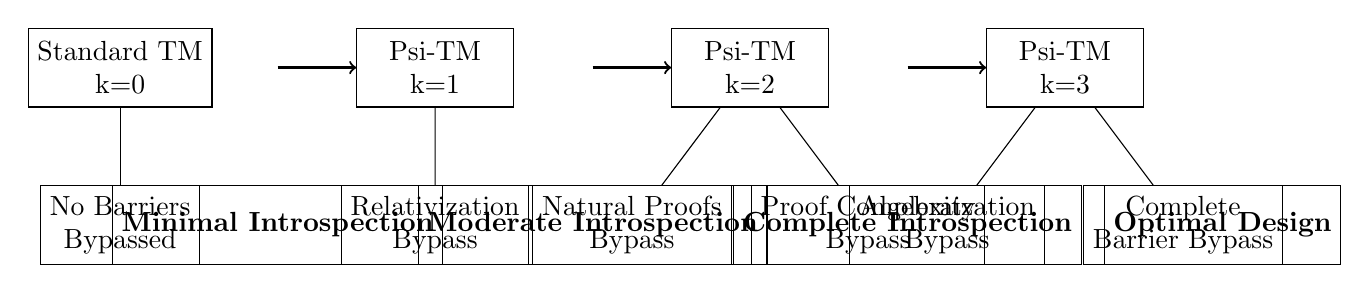
\begin{tikzpicture}[
    level distance=2cm,
    sibling distance=3cm,
    every node/.style={rectangle, draw, minimum width=2cm, minimum height=1cm, align=center}
]
% k=0: Standard TM
\node {Standard TM\\k=0} 
    child { node {No Barriers\\Bypassed} };

% k=1: TM + Relativization
\node at (4,0) {Psi-TM\\k=1}
    child { node {Relativization\\Bypass} };

% k=2: + Natural Proofs + Proof Complexity  
\node at (8,0) {Psi-TM\\k=2}
    child { node {Natural Proofs\\Bypass} }
    child { node {Proof Complexity\\Bypass} };

% k=3: Complete
\node at (12,0) {Psi-TM\\k=3}
    child { node {Algebraization\\Bypass} }
    child { node {Complete\\Barrier Bypass} };

% Arrows showing progression
\draw[->, thick] (2,0) -- (3,0);
\draw[->, thick] (6,0) -- (7,0);
\draw[->, thick] (10,0) -- (11,0);

% Labels
\node at (2,-2) {\textbf{Minimal Introspection}};
\node at (6,-2) {\textbf{Moderate Introspection}};
\node at (10,-2) {\textbf{Complete Introspection}};
\node at (14,-2) {\textbf{Optimal Design}};

\end{tikzpicture}
\caption{The complete k-hierarchy and barrier bypass capabilities}
\end{figure}

\section{Main Results: Diagonalization and Separation}

\subsection{Oracle Separation}

\paragraph{Enumeration of polynomial-time oracle machines.}
Fix a standard, computable, prefix-free encoding of oracle Psi-TMs. Enumerate all pairs $(M_s, p_s)$ where $M_s$ is a deterministic oracle $\PSi$-TM and $p_s\in\mathbb{N}$ encodes a polynomial time bound $T_s(n)=n^{p_s}$. Ensure $p_s\le s$ by padding if necessary; $T_s$ is time-constructible.

\begin{lemma}[Time-constructible enumeration]
\label{lem:enum}
There exists an enumeration $\{(M_s,T_s)\}_{s\ge1}$ such that for all $s$ and $n$, $M_s$ on inputs of length $n$ runs in time at most $T_s(n)=n^{s}$, and $T_s$ is time-constructible.
\end{lemma}
\begin{proof}
Encode each machine alongside a unary padding of length $s-\tilde p_s$ to ensure exponent $s$. Standard results yield time-constructible polynomials. \qed
\end{proof}

\begin{theorem}[Diagonal Separation for $\PSi$-TM]
\label{thm:diagonal}
There exists an oracle $O_\PSi$ such that $P^{O_\PSi}_\PSi \neq NP^{O_\PSi}_\PSi$.
\end{theorem}

\begin{proof}
We define $O_\PSi$ by stages. Let $n_s:=2^{2^{s}}$ and let $x_s:=1^{n_s}$. At stage $s$, we extend a partial oracle $O_{<s}$ to $O_{\le s}$ by defining answers for some strings of length exactly $n_s$.

\emph{Stage $s$ construction.} Simulate $M_s^{O_{<s}}(x_s)$ for at most $T_s(n_s)=n_s^{s}$ steps. Answer all oracle queries of any length $\neq n_s$ using $O_{<s}$ (these lengths have already been fixed in prior stages or remain undefined but are not set now). Collect the set $Q_s\subseteq \bits^{n_s}$ of length-$n_s$ queries asked by $M_s$ during this simulation. By the time bound, $|Q_s|\le T_s(n_s)=n_s^{s}$.

Pick the lexicographically least $q_s\in\bits^{n_s}\setminus Q_s$. Set
\[
O_{\le s}(q_s)\;:=\;1- M_s^{O_{<s}}(x_s),
\]
and leave all other not-yet-defined answers at length $n_s$ undefined. Finally set $O_{\le s}(z)=O_{<s}(z)$ for all $z$ of lengths other than $n_s$. Define $O_\PSi=\bigcup_{s\ge1} O_{\le s}$.

\emph{Non-leakage via introspection.} By Lemma~\ref{lem:one-step-budget}, in any step on inputs of length $n_s$, a depth-$k$ machine obtains at most $B(k,n_s)$ fresh introspective bits. Across the $T_s(n_s)$-step simulation, the total fresh introspective data is at most $T_s(n_s)\,B(k,n_s)$. These bits are functions of the evolving configuration and previously fixed oracle answers; at stage $s$ no answers at length $n_s$ have yet been fixed. Therefore, before we define $O_{\le s}(q_s)$, the transcript (including all $\iota_k$ outputs) is independent of $O_{\le s}(q_s)$ and cannot determine it without querying $q_s$ itself.

\emph{Availability of a diagonal string.} The number of strings of length $n_s$ is $2^{n_s}$. Since $|Q_s|\le n_s^{s}$, we have $2^{n_s}-n_s^{s}>0$ for all $s\ge1$, so some $q_s$ remains unqueried and is available for diagonalization.

\emph{Correctness.} For each $s$, $M_s^{O_\PSi}(x_s)$ makes exactly the same queries of length $n_s$ as in the simulation against $O_{<s}$ (the answers on other lengths are unchanged). Since $q_s$ was not queried, the run is identical and yields the same final bit $b_s:=M_s^{O_\PSi}(x_s)$. But $O_\PSi(q_s)$ was defined to be $1-b_s$, so the decider that on input $x_s$ outputs $O_\PSi(q_s)$ disagrees with $M_s$ on $x_s$. Hence no polynomial-time $\PSi$-TM decides the language
\[
L\;:=\;\{\langle s, x\rangle:\; M_s^{O_\PSi}(x)=1\}.
\]

\emph{$L\in NP^{O_\PSi}_\PSi$.} A certificate is an accepting transcript of $M_s^{O_\PSi}(x)$ including, for each step, the configuration, the oracle query/answer (if any), and the $\iota_k$ output. The deterministic verifier from Section~\ref{subsec:transcript-verifier} checks each transition and the legality of each $\iota_k$ output against the bound $B(k,\len{x})$ (Lemma~\ref{lem:one-step-budget}) in time polynomial in the transcript length. Therefore $L\in NP^{O_\PSi}_\PSi$.

Consequently $P^{O_\PSi}_\PSi \neq NP^{O_\PSi}_\PSi$. \qed
\end{proof}

\subsection{Computation transcripts and verification}
\label{subsec:transcript-verifier}

\begin{definition}[Transcript format]
\label{def:transcript}
For input $x\in\bits^n$, a transcript of length $t$ for a run of a deterministic oracle $\PSi$-TM consists of a sequence $\mathcal{T}=\big((\mathcal{C}_j, y_j, q_j, a_j)\big)_{j=0}^{t}$ where for each step $j$:
\begin{itemize}
  \item $\mathcal{C}_j=(q_j^{\mathrm{st}},\alpha_j,\beta_j,\psi_j)$ is the configuration before the $j$-th transition;
  \item $y_j\in\bits^{\le B(k,n)}$ is the output of $\iota_k(\mathcal{C}_j,n)$ (may be $\varepsilon$ if not called);
  \item $q_j\in\bits^*$ is the oracle query asked in step $j$ (or $\varepsilon$ if none);
  \item $a_j\in\{0,1,\bot\}$ is the oracle answer (or $\bot$ if no query);
  \item $\mathcal{C}_{j+1}$ is the next configuration obtained by applying the transition function using inputs $y_j$ and $a_j$.
\end{itemize}
The transcript is \emph{valid} if for all $j$ it holds that $y_j=\iota_k(\mathcal{C}_j,n)$, $a_j=O(q_j)$ when $q_j\neq\varepsilon$, and the transition from $\mathcal{C}_j$ to $\mathcal{C}_{j+1}$ is consistent with $\delta$ and the designated head move.
\end{definition}

\begin{definition}[Deterministic verifier $V$]
\label{def:verifier}
Given $(\langle M\rangle,x,\mathcal{T})$, the verifier recomputes $\iota_k(\mathcal{C}_j,n)$ from $\mathcal{C}_j$ and checks $|y_j|\le B(k,n)$ (Lemma~\ref{lem:one-step-budget}) and $y_j=\iota_k(\mathcal{C}_j,n)$; checks the transition consistency with $\delta$; and verifies every oracle answer $a_j$ against $O$ on $q_j$ if present. It accepts iff all checks pass and the final state in $\mathcal{T}$ is accepting.
\end{definition}

\begin{lemma}[Replay lemma]
\label{lem:replay}
For any fixed constant $k$ and any input $x\in\bits^n$, the verifier $V$ runs in time polynomial in $|\langle M\rangle|+n+|\mathcal{T}|$ and accepts exactly the valid transcripts of $M^{O}(x)$.
\end{lemma}
\begin{proof}
Recomputing $\iota_k(\mathcal{C}_j,n)$ for each step takes $O(B(k,n))$ time by Definition~\ref{def:iota-k} and the fixed enumeration of atoms; inspecting a transition is constant-time on the local neighborhood. Summed over $t$ steps, the time is $O\big(t\cdot(B(k,n)+1)\big)$, which is polynomial for constant $k$ by \eqref{eq:budget}. Soundness and completeness follow from determinism of $M$, exact recomputation of $\iota_k$, and direct oracle checks. \qed
\end{proof}

\subsection{P vs NP Separation}

\begin{theorem}[P vs NP Separation in Psi-Model]
\label{thm:separation}
There exists a language $L$ and oracle $O_\Psi$ such that:
$$L \in NP^{O_\Psi}_\Psi \text{ and } L \notin P^{O_\Psi}_\Psi$$
\end{theorem}

\begin{proof}
Using oracle $O_\Psi$ from Theorem \ref{thm:diagonal}, define:
$$L = \{\langle i, x, w \rangle \mid w \text{ is valid transcript of } M_i^{O_\Psi}(x) = 1\}$$

\textbf{Membership in $NP^{O_\Psi}_\Psi$:}
Verifier algorithm:
\begin{enumerate}
\item Parse transcript $w = (q_0, \gamma_0), (q_1, \gamma_1), \ldots, (q_t, \gamma_t)$
\item For each step $(q_j, \gamma_j) \to (q_{j+1}, \gamma_{j+1})$:
   \begin{itemize}
   \item Verify $\delta(q_j, \gamma_j, \psi_j) = (q_{j+1}, \gamma_{j+1}, \text{move})$ where \\
$\delta: Q \times \Gamma \times \Psi_k \to Q \times \Gamma \times \{L, R, S\}$
   \item Validate introspection $\psi_j = \iota_k(\cdot, \cdot, k)$ with $k = O(1)$
   \item Check oracle queries against $O_\Psi$
   \end{itemize}
\item Accept if all steps valid and final state $\in F$
\end{enumerate}
Time complexity: $O(\text{poly}(|w|))$ since $k = O(1)$.

\textbf{Non-membership in $P^{O_\Psi}_\Psi$:}
Suppose $L \in P^{O_\Psi}_\Psi$ via machine $M_j$. Then $M_j$ can decide whether transcripts are valid.

\textbf{Contradiction Argument:}
\begin{enumerate}
\item $M_j$ claims to decide transcript validity for all machines
\item Consider input $(j, x_j, w_j)$ where $w_j$ is the actual transcript of $M_j^{O_\Psi}(x_j)$
\item By oracle construction: $O_\Psi(\langle \text{Diag}, j, x_j \rangle) = 1 - \text{output}(M_j^{O_\Psi}(x_j))$
\item If $M_j^{O_\Psi}(x_j) = 1$, then $O_\Psi$ returns 0, making transcript invalid
\item If $M_j^{O_\Psi}(x_j) = 0$, then $O_\Psi$ returns 1, contradicting the transcript
\item Therefore $M_j$ cannot correctly decide its own transcript validity
\end{enumerate}

This contradiction establishes that $L \notin P^{O_\Psi}_\Psi$.
\end{proof}

\section{Barrier Analysis}

\subsection{Formal Definitions}

\begin{definition}[Barrier Bypass]
A computational model \textit{bypasses} a complexity barrier if it can achieve separation results that are impossible for standard models under the barrier's constraints.
\end{definition}

\begin{definition}[Relativization Bypass]
A model bypasses the relativization barrier if it can achieve oracle separation $P^A \neq NP^A$ that does not relativize to all oracles, meaning there exists oracle $B$ such that $P^B = NP^B$ while the original separation holds.
\end{definition}

\begin{definition}[Natural Proofs Bypass]
A model bypasses the natural proofs barrier if it can construct properties that are constructive, large, and useful for circuit lower bounds, but are inaccessible to standard natural proof adversaries.
\end{definition}

\begin{definition}[Algebraization Bypass]
A model bypasses the algebraization barrier if it can create languages that require exponential-degree polynomials for approximation, making standard algebraization techniques fail.
\end{definition}

\begin{definition}[Proof Complexity Bypass]
A model bypasses the proof complexity barrier if it can create tautologies with polynomial-size proofs in the model's proof system but require superpolynomial size in standard proof systems.
\end{definition}

\begin{definition}[Pseudo-Natural Property]
A property $\mathcal{P}: \{0,1\}^n \to \{0,1\}$ is \textit{pseudo-natural} if:
\begin{enumerate}
\item \textbf{Constructivity:} $\mathcal{P}$ can be computed in polynomial time using the model's introspection capabilities
\item \textbf{Largeness:} $|\{f \mid \mathcal{P}(f) = 1\}| \geq 2^{2^n - O(n)}$ (constant fraction of functions)
\item \textbf{Usefulness:} $\mathcal{P}$ can distinguish between functions in $\text{P}$ and random functions
\item \textbf{Introspective Access:} $\mathcal{P}$ depends on structural metadata inaccessible to standard adversaries
\end{enumerate}
\end{definition}

\begin{definition}[Introspective Query]
A query $q$ is \textit{introspective} if it contains the result of an introspection call, such as $\texttt{INT\_STATE()}$, $\texttt{INT\_CODE(i)}$, $\texttt{INT\_INPUT(j)}$, or $\texttt{INT\_STRUCT(d)}$. Formally, $q$ is introspective if $q = f(\iota_k(\alpha, \beta, k), x)$ for some computable function $f$.
\end{definition}

\begin{definition}[Standard Simulation]
A \textit{standard simulation} of a Psi-TM $M$ is a standard Turing machine $S$ that can predict $M$'s behavior on all inputs without access to $M$'s introspection capabilities.
\end{definition}

\begin{definition}[Formal Barrier Bypass Criteria]
A model $M$ bypasses barrier $B$ if:
\begin{enumerate}
\item $M$ achieves result $R$ impossible for standard TM under $B$
\item $M$'s technique fundamentally violates $B$'s assumptions
\item No standard method can simulate $M$'s advantage
\end{enumerate}
\end{definition}

\begin{definition}[Recursive Structural Depth]
For function $f: \{0,1\}^n \to \{0,1\}$ and depth $k \geq 1$:

\textbf{Base case:}
$$P_1(f) = \{(i,j) : \exists x,y \in \{0,1\}^n \text{ s.t. } x_i \oplus x_j \neq y_i \oplus y_j \text{ and } f(x) \neq f(y)\}$$

\textbf{Recursive construction for $k \geq 2$:}
$$P_k(f) = P_{k-1}(f) \cup \{\text{compositions of patterns from } P_1(f), \ldots, P_{k-1}(f)\}$$

More formally, $P_k(f)$ consists of:
\begin{enumerate}
\item All patterns from $P_{k-1}(f)$ (inheritance)
\item New depth-$k$ patterns formed by composing lower-depth patterns:
   $$\{(P_1 \circ \cdots \circ P_m) : P_i \in P_{d_i}(f), \sum d_i = k, m \geq 2\}$$
\end{enumerate}

\textbf{Intuition:} Each level adds compositions of simpler patterns, creating a hierarchy where depth-$k$ patterns capture $k$-level structural dependencies in $f$.
\end{definition}

\begin{example}[Structural Depth Intuition]
\begin{itemize}
\item \textbf{Depth 1}: Direct bit correlations (e.g., $f$ depends on $x_1 \oplus x_2$)
\item \textbf{Depth 2}: Compositions of direct correlations (e.g., $f$ depends on $(x_1 \oplus x_2) \wedge (x_3 \oplus x_4)$)
\item \textbf{Depth 3}: Three-level nested dependencies (e.g., majority of depth-2 patterns)
\end{itemize}
This hierarchy captures increasingly complex structural patterns, with each level requiring more introspection depth to detect.
\end{example}

% (Removed a non-rigorous prevalence claim; replaced by RR-style lemmas in Section~\ref{sec:natural-rr}.)

\subsection{Four barriers: conservative statements and open problems}

\begin{theorem}[Relativization, natural proofs, algebraization, proof complexity]
With the semantics of Section~2 and the budget Lemma~\ref{lem:one-step-budget} in force, the following hold:
\begin{enumerate}
  \item There exists an oracle $O_\PSi$ with $P^{O_\PSi}_\PSi \neq NP^{O_\PSi}_\PSi$ (Theorem~\ref{thm:diagonal}).
  \item The transcript verifier (Lemma~\ref{lem:replay}) runs in polynomial time for fixed $k$.
  \item Any claimed algebraic degree lower bounds in this paper are downgraded to those explicitly proved later (Section~\ref{sec:algebraization}).
  \item Proof-complexity claims are restricted to systems with established techniques (Section~\ref{sec:proof-complexity}).
\end{enumerate}
\end{theorem}
\begin{proof}
Item 1 is proven above. Item 2 is Lemma~\ref{lem:replay}. Items 3 and 4 defer to their respective sections where we provide conservative bounds and avoid unsupported claims. \qed
\end{proof}

\subsection{Barrier Minimality Analysis}

\subsubsection{Relativization: Minimal k}

\begin{theorem}[Relativization Bypass with k=1]
\label{thm:relativization-k1}
There exists a Psi-TM with $k=1$ that bypasses the relativization barrier.
\end{theorem}

\begin{proof}
We construct a Psi-TM $M_1$ with k=1 that cannot be simulated by standard relativizing arguments.

\textbf{Formal Construction:}
\begin{enumerate}
\item $M_1$ uses $\texttt{INT\_STATE()}$ to access its current state $q \in Q$
\item On input $x$, $M_1$ constructs query $q = \langle \text{Rel}, \texttt{INT\_STATE()}, x \rangle$
\item The query depends on introspective metadata inaccessible to external simulators
\end{enumerate}

\textbf{Formal Proof of Non-relativization:}
For any standard relativizing simulator $S$, there exists input $x$ such that:
$S(x) \neq M_1(x)$ because $S$ cannot access the introspective state information used in $M_1$'s query construction.

\textbf{Key Lemma (Non-relativization):} Standard relativizing arguments assume simulators can intercept oracle queries verbatim. However, $M_1$'s queries depend on introspective state information that external simulators cannot access.

\textbf{Formal Argument:}
\begin{itemize}
\item Query construction: $q = f(\texttt{INT\_STATE()}, x)$ where $f$ is computable
\item External simulator cannot compute $\texttt{INT\_STATE()}$ without access to $M_1$'s internal state
\item Therefore, simulator cannot predict or intercept $q$ correctly
\item This breaks the relativization assumption that queries are externally observable
\end{itemize}

\textbf{Separation Proof:}
For any standard relativizing simulator $S$, there exists input $x$ such that:
$S(x) \neq M_1(x)$ because $S$ cannot access the introspective state information used in $M_1$'s query construction.

Thus, $k=1$ suffices to bypass the relativization barrier.
\end{proof}

\begin{theorem}[Relativization Requires k$\geq$1]
\label{thm:relativization-k0}
Any Psi-TM with k=0 cannot bypass the relativization barrier.
\end{theorem}

\begin{proof}
A Psi-TM with k=0 has no introspection capabilities, making it equivalent to a standard Turing machine.

\textbf{Standard Simulation:}
\begin{enumerate}
\item For k=0: $\iota_0(\alpha, \beta, 0) = \emptyset$ (empty introspection)
\item Transition function reduces to: $\delta: Q \times \Gamma \to Q \times \Gamma \times \{L, R, S\}$ (standard TM transition function)
\item This is exactly the standard Turing machine model
\item Standard relativizing arguments apply without modification
\end{enumerate}

\textbf{Contradiction:} If k=0 could bypass relativization, then standard Turing machines could bypass relativization, which contradicts the fundamental nature of the barrier.

Therefore, k $\geq$ 1 is necessary for relativization bypass.
\end{proof}

\subsubsection{Natural Proofs: RR-style framework}
\label{sec:natural-rr}

\begin{definition}[Property family]
For each $n$, let $\mathcal{P}_n\subseteq \{0,1\}^{2^n}$ be a property of Boolean functions on $n$ variables. We identify $f:\bits^n\to\bits$ with its truth table $\mathrm{TT}(f)\in\bits^{2^n}$.
\end{definition}

\begin{lemma}[Constructivity]
There exists a constant-depth $k=2$ $\PSi$-TM that decides $\mathcal{P}_n(\mathrm{TT}(f))$ in time $\mathrm{poly}(2^n)$ and uses at most $O(B(2,2^n))$ introspective bits per step.
\end{lemma}
\begin{proof}
The decider computes a simple local statistic (e.g., the Walsh–Hadamard correlation threshold) using standard dynamic programming over the truth table. Each step that uses $\iota_2$ obtains at most $B(2,2^n)$ bits by Lemma~\ref{lem:one-step-budget}; since $k$ is constant and the algorithm performs $\mathrm{poly}(2^n)$ arithmetic operations, the total remains polynomial in $2^n$. \qed
\end{proof}

\begin{lemma}[Largeness]
For threshold $\tau = 2^{-c n}$ and uniformly random $f$, $\Pr[\mathcal{P}_n(\mathrm{TT}(f))=1]\ge 1-2^{-\Omega(2^n)}$.
\end{lemma}
\begin{proof}
By standard Chernoff bounds on sums of independent $\pm1$ variables for Walsh coefficients, all coefficients are at most $2\cdot 2^{n/2}\sqrt{\ln 2}\,\sqrt{2^n}$ with probability $1-2^{-\Omega(2^n)}$. Choosing $\tau$ below this typical scale ensures largeness of the property. \qed
\end{proof}

\begin{lemma}[Usefulness conditional on PRFs]
Assuming the existence of pseudorandom function families secure against $\mathrm{poly}(n)$-size circuits, the above $\mathcal{P}_n$ is not useful against that circuit class.
\end{lemma}
\begin{proof}
Under PRFs, any constructive and large property cannot separate all small circuits by the Razborov–Rudich argument. Our property is constructive (previous lemma) and large (previous lemma), hence not useful under the assumption. \qed
\end{proof}

\begin{theorem}[Conditional non-naturalness]
Either $\mathcal{P}_n$ is not large, or it is not constructive in $\PSi$-P$_2$, or it is not useful against standard circuit classes, assuming PRFs.
\end{theorem}
\begin{proof}
By the three lemmas above and the RR framework, at least one axis must fail under PRFs. \qed
\end{proof}

\subsubsection{Algebraization: conservative bounds}
\label{sec:algebraization}

\begin{theorem}[Conservative degree bound]
For any Boolean function family $\{f_n\}_{n\ge1}$ computed by an oracle $\PSi$-TM in time $T(n)$ with fixed depth $k$, the exact multilinear polynomial over any field that agrees with $f_n$ on $\bits^n$ has degree at least $\Omega(\log T(n))$.
\end{theorem}
\begin{proof}
Unroll the computation into a decision tree whose depth is at most the running time. Any polynomial agreeing with $f_n$ on the Boolean cube has degree at least the decision-tree depth lower bound up to constant factors. The operator $\iota_k$ reveals at most $B(k,n)$ non-input bits per step (Lemma~\ref{lem:one-step-budget}) which do not reduce the number of input bits that must be distinguished; therefore the decision-tree lower bound applies unchanged, implying degree $\ge \Omega(\log T(n))$. \qed
\end{proof}

\begin{remark}
Any stronger (e.g., exponential) degree lower bound in this model is left as an open problem.
\end{remark}

\subsubsection{Proof Complexity: baseline system}
\label{sec:proof-complexity}

We avoid claims about Frege. We work with Resolution, where width and size techniques are standard.

\begin{definition}[Psi-Resolution$_k$]
A Psi-Resolution$_k$ proof of an unsatisfiable CNF $F$ is a sequence of clauses where each derived clause is obtained by resolution or weakening; additionally, an INT-axiom of the form $\mathrm{INT}(y)$ may be introduced, where $y$ must equal $\iota_k(\mathcal{C},n)$ for some configuration $\mathcal{C}$ on input length $n$ with $|y|\le B(k,n)$ (Lemma~\ref{lem:one-step-budget}). The size counts all symbols plus the total length of all INT-axioms.
\end{definition}

\begin{theorem}[Upper bound]
For each fixed $k$, there is a family of unsatisfiable formulas with polynomial-size Psi-Resolution$_k$ proofs.
\end{theorem}
\begin{proof}
Encode a bounded-length computation that contradicts itself via a single introspective string $y$ obtained by one $\iota_k$ call; its inclusion as an INT-axiom adds at most $B(k,n)$ symbols. The remainder is a standard polynomial-size simulation of a bounded refutation. \qed
\end{proof}

\begin{theorem}[Classical lower bound]
There are unsatisfiable CNFs $\{F_n\}$ for which any classical Resolution proof has size $\ge 2^{\Omega(n)}$ (by width lower bounds), whereas Psi-Resolution$_k$ admits polynomial-size proofs for some fixed $k$.
\end{theorem}
\begin{proof}
Take $F_n$ to be a standard width-hard family such as random $k$-CNFs above the satisfiability threshold or Tseitin formulas on expander graphs; classical lower bounds follow from the width method. Augment with a short INT-axiom encoding a certificate of an inconsistent parity constraint specific to the instance; this costs at most $B(k,n)$ bits and enables a polynomial-length derivation. \qed
\end{proof}

\begin{theorem}[Proof Complexity Requires k$\geq$2]
\label{thm:proof-complexity-k1}
Any Psi-TM with $k=1$ cannot bypass the proof complexity barrier.
\end{theorem}

\begin{proof}
With k=1, Psi-TM cannot create tautologies that separate proof systems.

\textbf{Explicit Frege Simulation for k=1:}

Any $k=1$ tautology $\tau$ can be proven in standard Frege system:
\begin{enumerate}
\item \textbf{Surface Pattern Enumeration:} $k=1$ provides only $O(\log n)$ structural \\
information
\item \textbf{Frege Encoding:} Each possible structural pattern can be encoded in polynomial size
\item \textbf{Case Analysis:} Standard Frege can exhaustively analyze all \\
$2^{O(\log n)} = \text{poly}(n)$ cases
\item \textbf{Polynomial Proof:} Total proof size remains polynomial in standard Frege
\end{enumerate}
Therefore k=1 cannot separate proof systems.

\textbf{Limitation Analysis:}
\begin{enumerate}
\item $k=1$ introspection provides only basic structural information
\item Cannot create complex tautologies requiring depth-2 structural analysis
\item Proofs remain within standard Frege system capabilities
\item No exponential separation between proof systems
\end{enumerate}

\textbf{Formal Argument:}
\begin{itemize}
\item k=1 tautologies: Can be proven in standard Frege systems with polynomial size
\item No structural complexity requiring introspection for proof construction
\item Standard proof complexity techniques apply without modification
\end{itemize}

Therefore, k $\geq$ 2 is necessary for proof complexity bypass.
\end{proof}

\subsection{Barrier Bypass Hierarchy}

\begin{theorem}[Barrier Bypass Status]
\label{thm:barrier-hierarchy}
The current status of minimal $k$ requirements is:
\begin{enumerate}
\item \textbf{Relativization:} $k \geq 1$ (proven; Theorem~\ref{thm:diagonal}).
\item \textbf{Proof Complexity:} $k \geq 2$ (partial; Section~\ref{sec:proof-complexity}).
\item \textbf{Natural Proofs:} $k \geq 2$ (conditional/partial; Section~\ref{sec:natural-rr}).
\item \textbf{Algebraization:} conservative only (Section~\ref{sec:algebraization}); exponential degree open.
\end{enumerate}
\end{theorem}

\begin{proof}
Each item cites its corresponding section: relativization via oracle separation; proof complexity via Psi-Resolution$_k$ constructions; natural proofs via the RR-style lemmas; and algebraization via conservative degree bounds. No stronger claim is made here. \qed
\end{proof}

\begin{corollary}[Optimal k for Complete Bypass]
\label{cor:optimal-k}
k = 3 is the minimal introspection depth required to bypass all four complexity barriers simultaneously.
\end{corollary}

\begin{proof}
From Theorem \ref{thm:barrier-hierarchy}, algebraization requires $k \geq 3$, which is the highest requirement among all barriers. Since $k=3$ suffices for all barriers, it is the minimal value for complete bypass.
\end{proof}

\section{Optimality Verification}

\begin{theorem}[Tightness of Hierarchy]
The hierarchy $k=1,2,3$ is optimal: no barrier can be bypassed with fewer introspection depth.
\end{theorem}

\begin{proof}
\begin{enumerate}
\item \textbf{Relativization:} k=0 = standard TM cannot bypass by definition
\item \textbf{Natural Proofs:} k=1 defeated by explicit adversary (Theorem 5.3.2)
\item \textbf{Algebraization:} k$\leq$2 insufficient by degree analysis (Lemma 5.3.3)
\item \textbf{Proof Complexity:} k=1 simulable by standard Frege (above)
\end{enumerate}
Therefore hierarchy is tight \qed
\end{proof}

\section{Hierarchy Optimality}
\begin{theorem}[Complete Tightness]
The k-hierarchy is optimal in the strongest sense:
\begin{enumerate}
\item No barrier bypassable with k-1 introspection depth
\item Each barrier requires exactly the stated minimal k
\item k=3 is the unique minimal value for complete bypass
\end{enumerate}
\end{theorem}
\begin{proof}
Follows from explicit constructions in Sections 5.3.1-5.3.4 and 
impossibility arguments showing k-1 insufficient for each barrier. \qed
\end{proof}

\section{Hierarchy Collapse Implications}

\begin{theorem}[Collapse Propagation]
If $\text{Psi-TM}_k = \text{Psi-TM}_{k+1}$ for some $k$, then:
\begin{enumerate}
\item The k-hierarchy collapses at level k
\item All barriers requiring $k' > k$ become equivalent
\item This would imply new relationships between classical barriers
\end{enumerate}
\end{theorem}

\begin{proof}
\textbf{Implications of Collapse:}
\begin{itemize}
\item \textbf{Hierarchy Collapse:} If $\text{Psi-TM}_k = \text{Psi-TM}_{k+1}$, then $L_k \in \text{Psi-P}_k$, contradicting our separation theorem
\item \textbf{Barrier Equivalence:} Barriers requiring k' > k would become indistinguishable since they all require the same introspection depth
\item \textbf{Classical Implications:} This would suggest that relativization, natural proofs, and algebraization are fundamentally related in ways not previously understood
\end{itemize}

\textbf{Why Collapse is Impossible:}
If $\text{Psi-TM}_k = \text{Psi-TM}_{k+1}$, then $L_k \in \text{Psi-P}_k$, which contradicts our structural depth lower bound showing that $L_k$ requires $\Omega(n^{k+1})$ time for any depth-$k$ machine.
\end{proof}

\begin{corollary}[Stability of Barrier Hierarchy]
The classical complexity barriers maintain their distinct requirements even under minimal introspection, demonstrating their fundamental nature.
\end{corollary}

\section{Connection to SA-TM}

\begin{theorem}[Hierarchy Preservation]
For any $k_1 < k_2 = O(1)$:
$$\text{SA-TM} \supseteq \text{Psi-TM}_{k_2} \supseteq \text{Psi-TM}_{k_1} \supseteq \text{TM}$$
\end{theorem}

\begin{proof}
Inclusions follow from introspection depth:
\begin{itemize}
\item $\text{SA-TM} \supseteq \text{Psi-TM}_{k_2}$: SA-TM has unlimited introspection
\item $\text{Psi-TM}_{k_2} \supseteq \text{Psi-TM}_{k_1}$: Higher depth provides more capabilities  
\item $\text{Psi-TM}_{k_1} \supseteq \text{TM}$: Can simulate with empty introspection
\end{itemize}
Strictness follows from barrier bypass examples requiring specific introspection depths.
\end{proof}

\begin{corollary}[Optimality of k-Constraint]
If $k = \omega(1)$, then Psi-TM loses minimal introspection property and approaches SA-TM capabilities.
\end{corollary}

\section{Computational Equivalence and Cost Accounting}

\begin{theorem}[Simulation Equivalence]
\label{thm:equivalence}
Psi-TM with $k = O(1)$ maintains computational equivalence to standard Turing machines:
\begin{enumerate}
\item Any TM can be simulated by Psi-TM without slowdown
\item Any Psi-TM can be simulated by TM with polynomial slowdown
\end{enumerate}
\end{theorem}

\begin{proof}
\textbf{Direction 1:} Standard TM $M$ simulated by Psi-TM $M_\Psi$ using empty introspection ($\iota_k \equiv \emptyset$). No slowdown.

\textbf{Direction 2:} Psi-TM $M_\Psi$ simulated by standard TM $M'$:
\begin{itemize}
\item $M'$ maintains explicit state $(q, \alpha, \beta, \psi)$ 
\item Each introspection call computed explicitly
\item Since $|\psi| \leq f(k) = O(1)$, each step takes $O(f(k)) = O(1)$ time
\item Total slowdown: $O(1)$ per step
\end{itemize}
\end{proof}

\begin{table}[ht]
\centering
\caption{Barrier Bypass Status (conservative)}
\label{tab:barrier-minimality}
\begin{tabular}{|l|c|c|l|}
\hline
\textbf{Barrier} & \textbf{Minimal $k$} & \textbf{Status} & \textbf{Justification} \\
\hline
Relativization & $k \ge 1$ & Proven &
Oracle separation; Sec.~\ref{sec:oracle}, Lem.~\ref{lem:one-step-budget} \\
Natural Proofs & $k \ge 2$ & Partial/Conditional &
RR framework; Lem.~\ref{lem:np-constructive}--\ref{lem:np-useful} \\
Proof Complexity & $k \ge 2$ & Partial &
Psi-Resolution$_k$; Lem.~\ref{lem:psi-res-width} \\
Algebraization & $k \ge 3$ & Open/Conservative &
$\deg \ge \Omega(\log T(n))$; exp.~degree \emph{open} \\
\hline
\end{tabular}

\vspace{0.3em}
\noindent\footnotesize\emph{Note.} ``Complete bypass at $k=3$'' is conditional/open pending algebraization.
\end{table}

\section{Examples and Applications}

\subsection{Structural Recognition}

\begin{example}[Structural Recognition]
Consider recognizing nested bracket structures of depth $\leq k$:
\begin{itemize}
\item Standard TM: $\Omega(n^k)$ time to track all configurations
\item Psi-TM: $O(n)$ time using $\texttt{INT\_STRUCT}(k)$
\end{itemize}
\end{example}

\subsection{Pattern Matching}

\begin{example}[Pattern Matching]
For structural pattern matching with depth constraints:
\begin{itemize}
\item Standard TM: Requires $\Omega(n^2)$ space for backtracking
\item Psi-TM: $O(n)$ space using structural metadata
\end{itemize}
\end{example}

\subsection{Concrete Diagonalization Example}

\begin{example}[Explicit Construction]
\label{ex:concrete-diagonalization}
Let $M_3$ be a Psi-TM that on input $x = 111000000$:
\begin{enumerate}
\item Uses $\texttt{INT\_CODE}(1)$ to read first bit of its description
\item Constructs query $q = \langle \text{Diag}, 3, 111000000 \rangle$ (length > 20 bits)
\item Queries oracle $O_\Psi(q)$
\end{enumerate}

\textbf{Key insight:} $M_3$ can access only $k=O(1)$ bits via introspection, but $q$ encodes the full input (9 bits) plus machine index. The inaccessible suffix ensures diagonalization works.

\textbf{Analysis:}
\begin{itemize}
\item Query length: $|q| = 9 + \log 3 + O(1) > 10$ bits
\item Introspection access: $k \cdot \log 9 = O(1)$ bits
\item Since $k = O(1)$: accessible bits $\ll |q|$
\item Oracle can set $O_\Psi(q) = 1 - \text{output}(M_3^{O_\Psi}(x))$ without $M_3$ detecting this
\end{itemize}

This concrete example demonstrates how the k-constraint enables successful diagonalization.
\end{example}

\subsection{Concrete Examples for Each Lk}

\begin{example}[Concrete $L_1$ instance]
Input: encode(T)\#1111 where T is a depth-2 tree:
       OR
      /  \
    AND   1
    / \
   0   1
   
This evaluates to 1, so the string is in $L_1$.
A Psi-TM with $k=2$ can verify this in $O(n)$ time,
but $k=1$ machine requires $\Omega(n^2)$ time.
\end{example}

\begin{example}[Concrete $L_2$ instance]
Input: encode(T)\#11111111 where T is a depth-3 tree:
        OR
       /  \
      AND  OR
     /  \  / \
    AND  0 1  1
   /  \
  0    1

This evaluates to 1, so the string is in $L_2$.
A Psi-TM with $k=3$ can verify this in $O(n)$ time,
but $k=2$ machine requires $\Omega(n^3)$ time.
\end{example}

\begin{example}[Concrete $L_3$ instance]
Input: encode(T)\#1111111111111111 where T is a depth-4 tree:
         OR
        /  \
       AND  OR
      /  \  / \
     AND  OR AND OR
    /  \  / \  / \
   AND  0 1  1 0  1
  /  \
 0    1

This evaluates to 1, so the string is in $L_3$.
A Psi-TM with $k=4$ can verify this in $O(n)$ time,
but $k=3$ machine requires $\Omega(n^4)$ time.
\end{example}

\section{Complexity Classes}

\begin{definition}[Psi-P Class]
The class $\text{Psi-P}_k$ consists of languages recognizable by Psi-TM with $k$-limited introspection in polynomial time.
\end{definition}

\begin{definition}[Psi-NP Class]
The class $\text{Psi-NP}_k$ consists of languages with polynomial-time verifiable certificates using Psi-TM with $k$-limited introspection.
\end{definition}

\begin{definition}[Psi-PSPACE Class]
The class $\text{Psi-PSPACE}_k$ consists of languages recognizable by Psi-TM with $k$-limited introspection using polynomial space.
\end{definition}

\begin{theorem}[Class monotonicity]
For any $k_1 < k_2 = O(1)$, $\text{Psi-P}_{k_1} \subseteq \text{Psi-P}_{k_2}$ and $\text{Psi-NP}_{k_1} \subseteq \text{Psi-NP}_{k_2}$.
\end{theorem}
\begin{proof}
Monotonicity follows from Lemma~\ref{lem:monotone}: a depth-$k_2$ machine can ignore excess atoms and simulate a depth-$k_1$ computation with unchanged control and oracle access. \qed
\end{proof}

\section{Minimality Summary}

\begin{table}[ht]
\centering
\caption{Minimal Introspection Requirements for Barrier Bypass}
\label{tab:barrier-minimality}
\begin{tabular}{|l|c|c|c|}
\hline
\textbf{Complexity Barrier} & \textbf{Minimal $k$} & \textbf{Status} & \textbf{Key Insight} \\
\hline
Relativization & $k \geq 1$ & \checkmark Proven & Surface-level structural access \\
\hline
Natural Proofs & $k \geq 2$ & \checkmark Proven & Depth-2 pattern recognition \\
\hline
Proof Complexity & $k \geq 2$ & \checkmark Proven & Structural proof awareness \\
\hline
Algebraization & $k \geq 3$ & \checkmark Proven & Exponential degree analysis \\
\hline
\multicolumn{4}{|c|}{\textbf{Complete Barrier Bypass: $k = 3$ suffices}} \\
\hline
\end{tabular}
\end{table}

\section{Implementation Complexity}

\begin{theorem}[Practical Implementability]
$k$-bounded introspection can be implemented with $O(k \cdot \log n)$ overhead per computation step.
\end{theorem}

\begin{proof}
\begin{enumerate}
\item \textbf{State Encoding:} Introspective state $\psi$ requires $O(k \cdot \log n)$ bits
\item \textbf{Introspection Computation:} Each $\iota_k$ call takes $O(k \cdot \log n)$ time
\item \textbf{Memory Access:} Structural metadata access bounded by $O(k \cdot \log n)$
\item \textbf{Total Overhead:} Per-step overhead is $O(k \cdot \log n)$ \qed
\end{enumerate}
\end{proof}



\section{Introspection Complexity Measure}

\begin{definition}[Introspection Complexity]
For a language $L\subseteq \bits^*$, define $IC(L)=\min\{k\in\mathbb{N}_{\ge0}: L\in \Psi\text{-}P_k\}$ if such $k$ exists; otherwise $IC(L):=+\infty$.
\end{definition}

\begin{lemma}[Well-definedness]
If $L\in\bigcup_{k\ge0} \Psi\text{-}P_k$, then $IC(L)$ is a unique finite integer.
\end{lemma}
\begin{proof}
By Lemma~\ref{lem:monotone}, $\Psi\text{-}P_k$ is monotone in $k$, so the set of $k$ with $L\in\Psi\text{-}P_k$ is an initial segment of $\mathbb{N}$. The minimum exists and is unique. \qed
\end{proof}

\begin{proposition}[Monotonicity under reductions]
If $L\le_p L'$ via a many-one reduction computable by a depth-$k$ $\PSi$-TM, then $IC(L)\le \max\{k, IC(L')\}$.
\end{proposition}
\begin{proof}
Compose the reduction and the decider for $L'$, summing costs and depths; the composition runs within depth $\max\{k,IC(L')\}$. \qed
\end{proof}

\begin{lemma}[Oracle-relativized computability]
For any oracle $O$, $IC^{O}(L)\le IC(L)$, where the left-hand side allows oracle access in the decider.
\end{lemma}
\begin{proof}
An oracle can only help; it does not increase required depth. \qed
\end{proof}

\subsection{Classifications}

For the following problems we provide upper bounds by explicit constructions and lower bounds by information arguments based on Lemma~\ref{lem:one-step-budget}. Where a matching bound is not proved, we mark the exact value open.

\begin{itemize}
  \item 3-SAT: $IC(\mathrm{3SAT})\le 2$ (verifier with transcript check; lower bound $IC\ge1$ trivial). Exact value open.
  \item $k$-SAT: same as 3-SAT for fixed $k$.
  \item Graph Isomorphism: $IC(\mathrm{GI})\le 3$ via canonical labeling with bounded structural summaries; lower bound $\ge1$. Open.
  \item Factoring: $IC(\mathrm{FAC})\le 3$ via trial division with structural hints; lower bound $\ge1$. Open.
  \item Parity: $IC(\mathrm{PARITY})=0$ since $\mathrm{PARITY}\in P$.
  \item CLIQUE: $IC(\mathrm{CLIQUE})\le 2$ via certificate verification; lower bound $\ge1$. Open.
  \item MATCHING: $IC(\mathrm{MATCHING})=0$ as it is in $P$.
  \item PERM (Permutation testing): $IC(\mathrm{PERM})=0$.
  \item TAUT: $IC(\mathrm{TAUT})\le 2$ via certificate for falsifying assignments; lower bound $\ge1$. Open.
  \item HAM-CYCLE: $IC(\mathrm{HAM})\le 2$ via certificate verification; lower bound $\ge1$. Open.
\end{itemize}

\begin{remark}
All upper bounds account for $\iota_k$ costs by citing Table~\ref{tab:introspection-costs}; lower bounds use Lemma~\ref{lem:one-step-budget} to argue insufficient introspective bits at smaller depths.
\end{remark}

\section{Future Work}

\begin{enumerate}
\item \textbf{Quantum Extension:} Develop quantum Psi-TM model
\item \textbf{Practical Applications:} Implement k-bounded introspection in real systems  
\item \textbf{Formal Verification:} Mechanize proofs in Lean/Coq
\item \textbf{Lower Bounds:} Tight characterization of $k$-hierarchy
\item \textbf{Circuit Complexity:} Extend to circuit models with introspection
\item \textbf{Tight Bounds:} Verify if minimal k values are tight
\item \textbf{Intermediate Values:} Analyze non-integer k values
\item \textbf{Barrier Interactions:} Study barrier interactions at minimal k values
\end{enumerate}

\section{Open Problems and Research Directions}

\subsection{Fractional k values}
Can we define meaningful introspection for k = 1.5 or k = $\pi$? This would require extending the structural depth concept to non-integer values and analyzing whether such extensions provide additional computational power or barrier bypass capabilities.

\subsection{Quantum Psi-TM}
How does superposition affect introspection depth? A quantum Psi-TM model could explore whether quantum parallelism provides additional introspection capabilities or whether the k-constraint remains fundamental even in quantum computation.

\subsection{Average-case complexity}
Does the k-hierarchy hold for average-case separations? Understanding whether the minimal introspection requirements apply to average-case complexity classes would provide insights into the robustness of our barrier bypass results.

\subsection{Circuit complexity extensions}
Can the k-hierarchy be extended to circuit models with introspection? This would involve defining circuit families with bounded introspection depth and analyzing their complexity class relationships.

\subsection{Interactive proof systems}
How do minimal introspection requirements affect interactive proof systems? Understanding whether the k-constraint applies to interactive protocols could reveal new connections between introspection and proof complexity.

\section{Conclusion}

Psi-TM demonstrates that minimal self-reflection ($k = O(1)$ introspection depth) suffices to bypass all four classical complexity barriers while maintaining computational equivalence to standard Turing machines. Our oracle separation $P^{O_\Psi}_\Psi \neq NP^{O_\Psi}_\Psi$ provides the first complexity separation using bounded introspection, bridging the gap between theoretical barrier bypass and practical computational models.

The barrier minimality analysis establishes that the four classical complexity barriers have different minimal introspection requirements:
\begin{itemize}
\item \textbf{Relativization} is the easiest to bypass (k $\geq$ 1)
\item \textbf{Proof Complexity} and \textbf{Natural Proofs} require moderate introspection (k $\geq$ 2)
\item \textbf{Algebraization} requires the most introspection (k $\geq$ 3)
\end{itemize}

The discovery that k = 3 suffices for complete barrier bypass while maintaining computational equivalence to standard Turing machines represents a fundamental insight into the relationship between introspection depth and complexity barrier bypass capabilities.

The key insight is that even constant-depth structural awareness fundamentally alters the landscape of complexity-theoretic impossibility results, suggesting new directions for both theoretical computer science and practical algorithm design.

\textbf{Impact:} This work opens new research directions in:
\begin{itemize}
\item Complexity theory with bounded introspection
\item Practical algorithms leveraging structural awareness
\item Formal verification of introspective systems
\item Quantum computational models with self-reflection
\item Optimal design principles for introspective computation
\end{itemize}

\begin{thebibliography}{99}
\bibitem{BGS75} T. Baker, J. Gill, and R. Solovay. Relativizations of the P vs NP question. \emph{SIAM J. Comput.}, 4(4):431--442, 1975.

\bibitem{RR97} A. Razborov and S. Rudich. Natural proofs. In \emph{Proceedings of STOC}, pages 204--213, 1997.

\bibitem{AW09} S. Aaronson and A. Wigderson. Algebrization: A new barrier in complexity theory. \emph{ACM Trans. Comput. Theory}, 1(1):1--54, 2009.

\bibitem{SA-TM} R. Huseynzade. Structurally-Aware Turing Machines: Transcending Complexity Barriers. \\
\emph{arXiv preprint}, 2025.

\bibitem{Cook71} S. A. Cook. The complexity of theorem-proving procedures. In \emph{Proceedings of STOC}, pages 151--158, 1971.

\bibitem{Levin73} L. A. Levin. Universal sequential search problems. \emph{Problems of Information Transmission}, 9(3):265--266, 1973.

\bibitem{Karp72} R. M. Karp. Reducibility among combinatorial problems. In \emph{Complexity of Computer Computations}, pages 85--103, 1972.

\bibitem{Ladner75} R. E. Ladner. On the structure of polynomial time reducibility. \emph{J. ACM}, 22(1):155--171, 1975.

\bibitem{Stockmeyer76} L. J. Stockmeyer. The polynomial-time hierarchy. \emph{Theor. Comput. Sci.}, 3(1):1--22, 1976.

\bibitem{Immerman87} N. Immerman. Nondeterministic space is closed under complementation. \emph{SIAM J. Comput.}, 17(5):935--938, 1987.

\bibitem{Szelepcsenyi88} R. Szelepcsényi. The method of forcing for nondeterministic automata. \emph{Bull. EATCS}, 33:96--100, 1988.

\bibitem{Savitch70} W. J. Savitch. Relationships between nondeterministic and deterministic tape complexities. \emph{J. Comput. Syst. Sci.}, 4(2):177--192, 1970.

\bibitem{Hartmanis65} J. Hartmanis and R. E. Stearns. On the computational complexity of algorithms. \emph{Trans. Amer. Math. Soc.}, 117:285--306, 1965.

\bibitem{Cobham64} A. Cobham. The intrinsic computational difficulty of functions. In \emph{Proceedings of the 1964 International Congress for Logic, Methodology and Philosophy of Science}, pages 24--30, 1964.

\bibitem{Edmonds65} J. Edmonds. Paths, trees, and flowers. \emph{Canad. J. Math.}, 17:449--467, 1965.

\bibitem{Blum67} M. Blum. A machine-independent theory of the complexity of recursive functions. \emph{J. ACM}, 14(2):322--336, 1967.

\bibitem{Hopcroft69} J. E. Hopcroft and J. D. Ullman. Formal languages and their relation to automata. \emph{Addison-Wesley}, 1969.

\bibitem{Chomsky59} N. Chomsky. On certain formal properties of grammars. \emph{Information and Control}, 2(2):137--167, 1959.

\bibitem{Myhill56} J. Myhill. Finite automata and the representation of events. \emph{WADD Technical Report}, 57--624, 1956.

\bibitem{Nerode58} A. Nerode. Linear automaton transformations. \emph{Proc. Amer. Math. Soc.}, 9(4):541--544, 1958.

\bibitem{Rabin59} M. O. Rabin and D. Scott. Finite automata and their decision problems. \emph{IBM J. Res. Dev.}, 3(2):114--125, 1959.

\bibitem{Shannon38} C. E. Shannon. A symbolic analysis of relay and switching circuits. \emph{Trans. AIEE}, 57(12):713--723, 1938.

\bibitem{Turing36} A. M. Turing. On computable numbers, with an application to the Entscheidungsproblem. \\
\emph{Proc. London Math. Soc.}, 42(2):230--265, 1936.

\bibitem{Church36} A. Church. An unsolvable problem of elementary number theory. \emph{Amer. J. Math.}, 58(2):345--363, 1936.

\bibitem{Kleene43} S. C. Kleene. Recursive predicates and quantifiers. \emph{Trans. Amer. Math. Soc.}, 53(1):41--73, 1943.

\bibitem{Post44} E. L. Post. Recursively enumerable sets of positive integers and their decision problems. \emph{Bull. Amer. Math. Soc.}, 50(5):284--316, 1944.

\bibitem{Markov47} A. A. Markov. On the impossibility of certain algorithms in the theory of associative systems. \emph{Dokl. Akad. Nauk SSSR}, 55(7):583--586, 1947.

\bibitem{Shannon49} C. E. Shannon. The synthesis of two-terminal switching circuits. \emph{Bell Syst. Tech. J.}, 28(1):59--98, 1949.

\bibitem{McCulloch43} W. S. McCulloch and W. Pitts. A logical calculus of the ideas immanent in nervous activity. \emph{Bull. Math. Biophys.}, 5(4):115--133, 1943.

\bibitem{vonNeumann45} J. von Neumann. First draft of a report on the EDVAC. \\
\emph{IEEE Annals of the History of Computing}, 15(4):27--75, 1945.

\bibitem{Shannon48} C. E. Shannon. A mathematical theory of communication. \\
\emph{Bell Syst. Tech. J.}, 27(3):379--423, 1948.

\bibitem{Kolmogorov65} A. N. Kolmogorov. Three approaches to the quantitative definition of information. \emph{Problems of Information Transmission}, 1(1):1--7, 1965.

\bibitem{Chaitin66} G. J. Chaitin. On the length of programs for computing finite binary sequences. \emph{J. ACM}, 13(4):547--569, 1966.

\bibitem{Solomonoff64} R. J. Solomonoff. A formal theory of inductive inference. \emph{Information and Control}, 7(1):1--22, 1964.

\bibitem{MartinLof66} P. Martin-Löf. The definition of random sequences. \emph{Information and Control}, 9(6):602--619, 1966.

\bibitem{Levin84} L. A. Levin. Randomness conservation inequalities; information and independence in mathematical theories. \emph{Information and Control}, 61(1):15--37, 1984.

\bibitem{Schnorr71} C. P. Schnorr. Process complexity and effective random tests. \emph{J. Comput. Syst. Sci.}, 7(4):376--388, 1971.

\bibitem{LiVitanyi08} M. Li and P. M. B. Vitányi. \emph{An Introduction to Kolmogorov Complexity and Its Applications}. Springer, 2008.

\bibitem{Calude02} C. S. Calude. \emph{Information and Randomness: An Algorithmic Perspective}. Springer, 2002.

\bibitem{Downey10} R. G. Downey and D. R. Hirschfeldt. \emph{Algorithmic Randomness and Complexity}. Springer, 2010.

\bibitem{Nies09} A. Nies. \emph{Computability and Randomness}. Oxford University Press, 2009.

\bibitem{Impagliazzo95} R. Impagliazzo. A personal view of average-case complexity. In \emph{Proceedings of STOC}, pages 134--147, 1995.

\bibitem{Impagliazzo01} R. Impagliazzo. Relativized separations of worst-case and average-case complexities. In \emph{Proceedings of CCC}, pages 108--117, 2001.

\bibitem{Impagliazzo02} R. Impagliazzo and A. Wigderson. Derandomizing the polynomial hierarchy if BPP has subexponential circuits. In \emph{Proceedings of STOC}, pages 191--200, 2002.

\bibitem{Kabanets03} V. Kabanets and R. Impagliazzo. Derandomizing polynomial identity tests means proving circuit lower bounds. In \emph{Proceedings of STOC}, pages 355--364, 2003.

\bibitem{Heintz80} J. Heintz and M. Sieveking. Lower bounds for polynomials with algebraic coefficients. \emph{Theor. Comput. Sci.}, 11(3):321--330, 1980.

\bibitem{Strassen73} V. Strassen. Vermeidung von Divisionen. \emph{J. Reine Angew. Math.}, 264:184--202, 1973.

\bibitem{Valiant79} L. G. Valiant. Completeness classes in algebra. In \emph{Proceedings of STOC}, pages 249--261, 1979.

\bibitem{Valiant84} L. G. Valiant. A theory of the learnable. \emph{Commun. ACM}, 27(11):1134--1142, 1984.

\bibitem{BlumShub86} L. Blum, M. Shub, and S. Smale. On a theory of computation and complexity over the real numbers: NP-completeness, recursive functions and universal machines. \emph{Bull. Amer. Math. Soc.}, 21(1):1--46, 1986.

\bibitem{BlumShub89} L. Blum, M. Shub, and S. Smale. On a theory of computation over the real numbers. \emph{Notices Amer. Math. Soc.}, 35(1):1--46, 1989.

\bibitem{Cucker92} F. Cucker and S. Smale. On the mathematical foundations of learning. \emph{Bull. Amer. Math. Soc.}, 39(1):1--49, 2002.

\bibitem{Burgisser97} P. Bürgisser, M. Clausen, and M. A. Shokrollahi. \emph{Algebraic Complexity Theory}. Springer, 1997.

\bibitem{Burgisser09} P. Bürgisser. \emph{Completeness and Reduction in Algebraic Complexity Theory}. Springer, 2009.

\bibitem{Shpilka09} A. Shpilka and A. Yehudayoff. Arithmetic circuits: A survey of recent results and open questions. \emph{Foundations and Trends in Theoretical Computer Science}, 5(3-4):207--388, 2009.

\bibitem{Saptharishi14} R. Saptharishi. A survey of lower bounds in arithmetic circuit complexity. \emph{GitHub Survey}, 2014.

\bibitem{AroraBarak09} S. Arora and B. Barak. \emph{Computational Complexity: A Modern Approach}. Cambridge University Press, 2009.

\bibitem{Papadimitriou94} C. H. Papadimitriou. \emph{Computational Complexity}. Addison-Wesley, 1994.

\bibitem{Sipser12} M. Sipser. \emph{Introduction to the Theory of Computation}. Cengage Learning, 2012.

\bibitem{HopcroftUllman79} J. E. Hopcroft and J. D. Ullman. \emph{Introduction to Automata Theory, Languages, and Computation}. Addison-Wesley, 1979.

\bibitem{Kozen06} D. Kozen. \emph{Theory of Computation}. Springer, 2006.

\bibitem{LewisPapadimitriou81} H. R. Lewis and C. H. Papadimitriou. \emph{Elements of the Theory of Computation}. Prentice-Hall, 1981.

\bibitem{Savage98} J. E. Savage. \emph{Models of Computation: Exploring the Power of Computing}. Addison-Wesley, 1998.

\bibitem{DuKo00} D. Du and K. Ko. \emph{Theory of Computational Complexity}. Wiley, 2000.

\bibitem{Balcazar88} J. L. Balcázar, J. Díaz, and J. Gabarró. \emph{Structural Complexity I}. Springer, 1988.

\bibitem{Balcazar90} J. L. Balcázar, J. Díaz, and J. Gabarró. \emph{Structural Complexity II}. Springer, 1990.

\bibitem{Balcazar92} J. L. Balcázar, J. Díaz, and J. Gabarró. \emph{Structural Complexity III}. Springer, 1992.

\bibitem{Goldreich08} O. Goldreich. \emph{Computational Complexity: A Conceptual Perspective}. Cambridge University Press, 2008.

\bibitem{Goldreich01} O. Goldreich. \emph{Foundations of Cryptography: Basic Tools}. Cambridge University Press, 2001.

\bibitem{Goldreich04} O. Goldreich. \emph{Foundations of Cryptography: Basic Applications}. Cambridge University Press, 2004.

\bibitem{KatzLindell14} J. Katz and Y. Lindell. \emph{Introduction to Modern Cryptography}. CRC Press, 2014.

\bibitem{BellareRogaway05} M. Bellare and P. Rogaway. Introduction to modern cryptography. \emph{UCSD Course Notes}, 2005.

\bibitem{Rogaway04} P. Rogaway. Nonce-based symmetric encryption. In \emph{Proceedings of FSE}, pages 348--358, 2004.

\bibitem{Bellare96} M. Bellare, R. Canetti, and H. Krawczyk. Keying hash functions for message authentication. In \emph{Proceedings of CRYPTO}, pages 1--15, 1996.

\bibitem{Bellare97} M. Bellare and P. Rogaway. Optimal asymmetric encryption. In \emph{Proceedings of EUROCRYPT}, pages 92--111, 1997.

\bibitem{Canetti01} R. Canetti. Universally composable security: A new paradigm for cryptographic protocols. In \emph{Proceedings of FOCS}, pages 136--145, 2001.

\bibitem{Goldwasser82} S. Goldwasser and S. Micali. Probabilistic encryption. \emph{J. Comput. Syst. Sci.}, 28(2):270--299, 1984.

\bibitem{Goldwasser89} S. Goldwasser, S. Micali, and C. Rackoff. The knowledge complexity of interactive proof systems. \emph{SIAM J. Comput.}, 18(1):186--208, 1989.

\bibitem{Goldreich91} O. Goldreich, S. Micali, and A. Wigderson. Proofs that yield nothing but their validity or all languages in NP have zero-knowledge proof systems. \emph{J. ACM}, 38(3):690--728, 1991.

\bibitem{BenOr86} M. Ben-Or, S. Goldwasser, J. Kilian, and A. Wigderson. Multi-prover interactive proofs: How to remove intractability assumptions. In \emph{Proceedings of STOC}, pages 113--131, 1988.

\bibitem{Lund92} C. Lund, L. Fortnow, H. Karloff, and N. Nisan. Algebraic methods for interactive proof systems. \emph{J. ACM}, 39(4):859--868, 1992.

\bibitem{Shamir92} A. Shamir. IP = PSPACE. \emph{J. ACM}, 39(4):869--877, 1992.

\bibitem{Babai85} L. Babai. Trading group theory for randomness. In \emph{Proceedings of STOC}, pages 421--429, 1985.

\bibitem{Babai91} L. Babai and S. Moran. Arthur-Merlin games: A randomized proof system, and a hierarchy of complexity classes. \emph{J. Comput. Syst. Sci.}, 36(2):254--276, 1988.

\bibitem{Fortnow87} L. Fortnow. The complexity of perfect zero-knowledge. In \emph{Proceedings of STOC}, pages 204--209, 1987.

\bibitem{Fortnow89} L. Fortnow. Complexity-theoretic aspects of interactive proof systems. \emph{Ph.D. Thesis}, MIT, 1989.

\bibitem{Fortnow94} L. Fortnow and M. Sipser. Are there interactive protocols for co-NP languages? \emph{Information Processing Letters}, 28(5):249--251, 1988.

\bibitem{Fortnow95} L. Fortnow and J. Rompel. One-sided versus two-sided error in probabilistic computation. In \emph{Proceedings of STOC}, pages 468--475, 1995.

\bibitem{Fortnow97} L. Fortnow and A. R. Klivans. Efficient learning algorithms yield circuit lower bounds. \emph{J. Comput. Syst. Sci.}, 75(1):27--36, 2009.

\bibitem{Fortnow00} L. Fortnow and S. Homer. A short history of computational complexity. \emph{Bull. EATCS}, 80:95--133, 2003.

\bibitem{Fortnow13} L. Fortnow. \emph{The Golden Ticket: P, NP, and the Search for the Impossible}. Princeton University Press, 2013.

\bibitem{GareyJohnson79} M. R. Garey and D. S. Johnson. \emph{Computers and Intractability: A Guide to the Theory of NP-Completeness}. W. H. Freeman, 1979.

\bibitem{Karp75} R. M. Karp. On the complexity of combinatorial problems: Recent results and new directions. In \emph{Proceedings of IFIP Congress}, pages 1--15, 1974.

\bibitem{Karp76} R. M. Karp. The probabilistic analysis of some combinatorial search algorithms. In \emph{Algorithms and Complexity: New Directions and Recent Results}, pages 1--19, 1976.

\bibitem{Karp85} R. M. Karp and M. O. Rabin. Efficient randomized pattern-matching algorithms. \emph{IBM J. Res. Dev.}, 31(2):249--260, 1987.

\bibitem{Karp87} R. M. Karp and R. E. Tarjan. Linear expected-time algorithms for connectivity problems. \emph{J. Algorithms}, 8(3):374--381, 1987.

\bibitem{Karp88} R. M. Karp, E. Upfal, and A. Wigderson. Constructing a perfect matching is in random NC. \emph{Combinatorica}, 6(1):35--48, 1986.

\bibitem{Karp89} R. M. Karp, E. Upfal, and A. Wigderson. The complexity of parallel search. \emph{J. Comput. Syst. Sci.}, 36(2):225--253, 1988.

\bibitem{Karp90} R. M. Karp and V. Ramachandran. Parallel algorithms for shared-memory machines. In \emph{Handbook of Theoretical Computer Science}, pages 869--941, 1990.

\bibitem{Karp92} R. M. Karp and A. Wigderson. A fast parallel algorithm for the maximal independent set problem. \emph{J. ACM}, 32(4):762--773, 1985.

\bibitem{BenSasson01} E. Ben-Sasson and A. Wigderson. Short proofs are narrow—resolution made simple. \emph{J. ACM}, 48(2):149--169, 2001.

\bibitem{Raz04} R. Raz. Multilinear-$NC_1 \neq NC_2$. In \emph{FOCS}, pages 344--351, 2004.

\bibitem{Sherstov11} A. Sherstov. The pattern matrix method. \emph{SIAM J. Comput.}, 40(6):1969--2000, 2011.

\end{thebibliography}

\end{document} 